\chapter{System Overview}

\begin{figure}
\center
	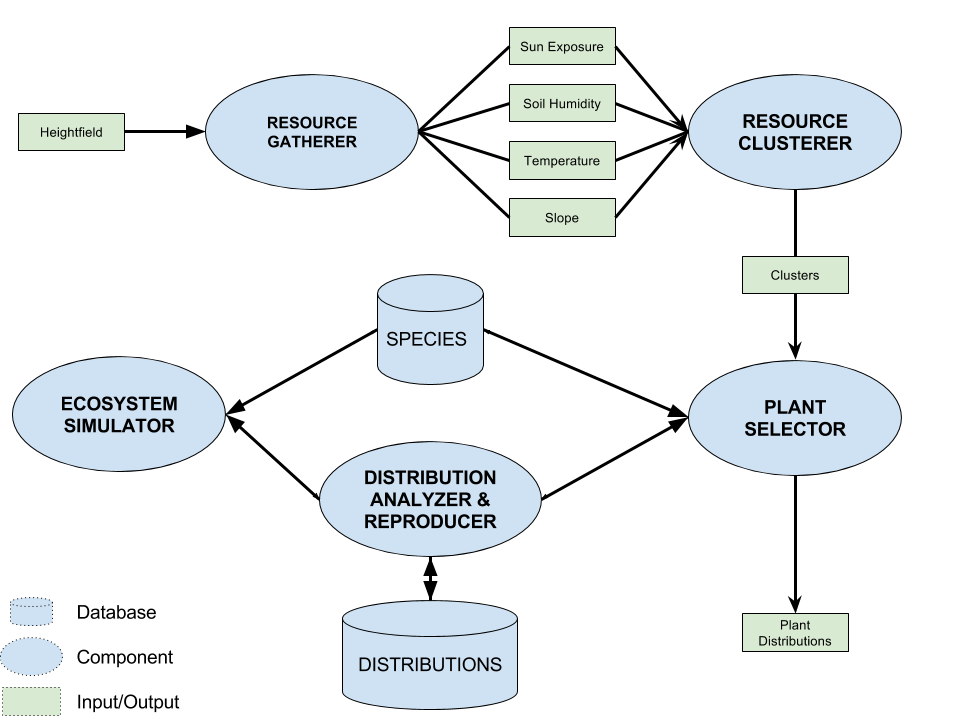
\includegraphics[width=\textwidth]{system_overview.png}
	\caption{ System overview}	
	\label{fig:system_overview}
\end{figure}

Multiple components serving specific purposes constitute the building blocks of the overall system, notably: \textit{resource gathering}, \textit{resource clustering}, \textit{plant selection}, \textit{ecosystem simulation} and \textit{distribution analysis and reproduction}. The purpose of this chapter is to give an overview of the system, each component and how they fit together (as illustrated in figure \ref{fig:system_overview}). To do so, an overview of each component is provided separately along with it's purpose, required inputs and outputs. To conclude this chapter, the \textit{limitations} of the system will be discussed. \\

\section{Resource Gatherer}

Vegetation requires resources to grow and the distribution of these resources identifies a given species and associated it with a given climate and, subsequently, location on earth. Determining resource data is essential, therefore, to generating realistic virtual worlds as it is vital to determining vegetation distribution patterns. The purpose of the resource gatherer is to determine, for each terrain vertex: \textit{sun exposure}, \textit{soil humidity}, \textit{temperature} and \textit{slope}. Figure \ref{fig:system_overview_resource_gatherer} illustrates the output of the resource gatherer along with the user inputs required.\\
The latitude and orientation of the terrain must be specified by the user in order to determine the sun position throughout the year. The \textit{sunlight exposure} calculation then determines, given this information and the terrain relief, the average daily illumination (in hours) received by each terrain vertex for each month of the year. To calculate the average illumination for a given month, the trajectory of the sun is calculated for the fifteenth day. \\
In order to calculate the \textit{soil humidity} for each month, the soil infiltration rate, monthly rainfall quantity and monthly rainfall intensity must be configured.\\
To determine the \textit{temperature} of each terrain vertex, the user must specify the temperature at zero metres in June and December along with the associated lapse rate. These temperatures are then considered the annual minimum and maximum and are used to deduce the temperature for any month through linear interpolation. The lapse rate represents the decrease in temperature with altitude and is used to determine the temperature for any terrain vertex given its altitude. \\
The \textit{slope} is determined automatically from the input terrain.\\

\begin{figure}
\center
	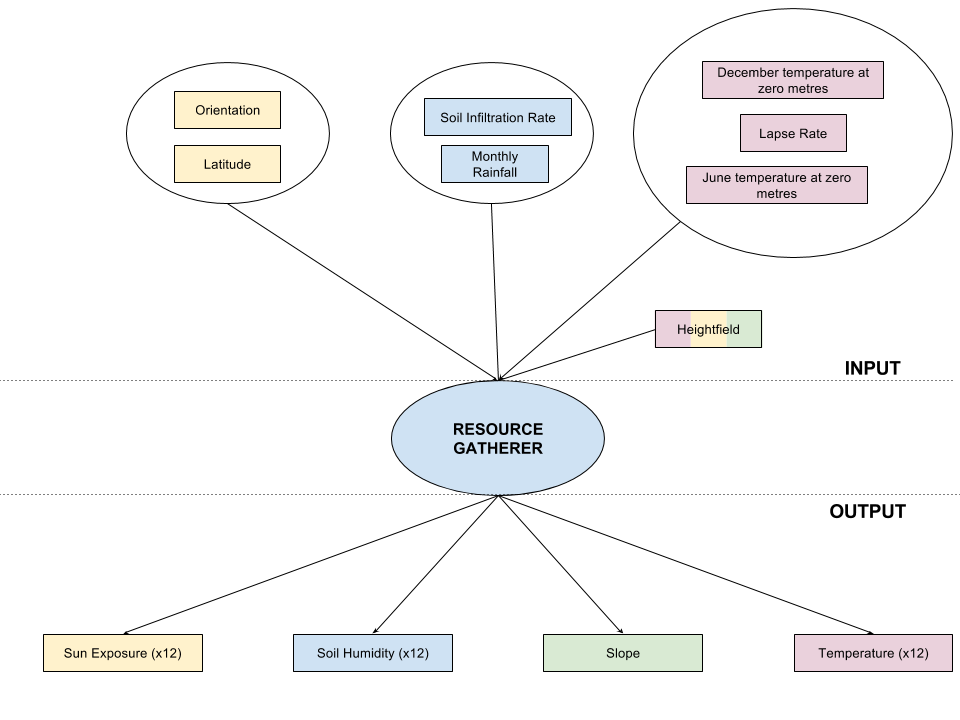
\includegraphics[scale=0.3]{system_overview_resource_gatherer.png}
	\caption{ Resource gatherer overview with colour coding to correlate input with corresponding output.}	
	\label{fig:system_overview_resource_gatherer}
\end{figure}

\section{Resource Clusterer}

Determining a suitable plant distribution for each individual terrain vertex is infeasible due to the associated computational cost. To reduce the amount of plant distributions to calculate, K-means clustering is performed on the terrain to group together points with similar resource properties. The mean value of each cluster is then used to determine suitable vegetation and distribution thereof. Figure \ref{fig:system_overview_resoure_clusterer} illustrates the input requirements and output of this component.

\begin{figure}
\center
	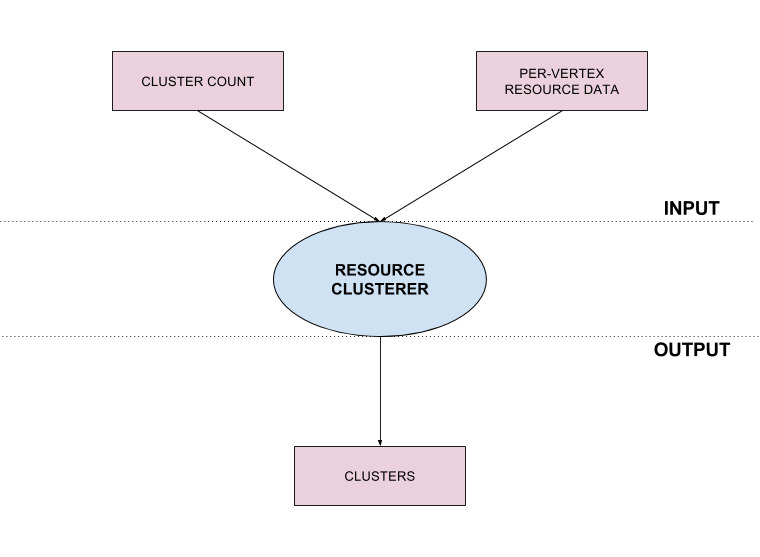
\includegraphics[scale=0.3]{system_overview_resource_clusterer.png}
	\caption{ Resource clusterer overview.}	
	\label{fig:system_overview_resoure_clusterer}
\end{figure}

\section{Plant Selector}

Given the mean value of the individual clusters, the plant selector determines the plants which are able to survive in each terrain cluster and calculates for each of them a suitability score. This score depicts how suited a specie is to each individual cluster and is illustrated to the user for informational purposes in order to facilitate the specie selection procedure. Figure \ref{fig:system_overview_plant_selector} shows the input requirements and outputs of this component.

\begin{figure}
\center
	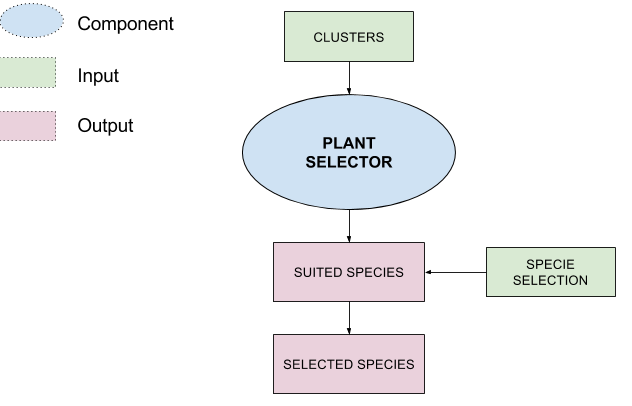
\includegraphics[scale=0.3]{system_overview_plant_selector.png}
	\caption{ Plant selector overview.}	
	\label{fig:system_overview_plant_selector}
\end{figure}

\section{Ecosystem Simulator}

The ecosystem simulator is used to determine a valid plant distribution given a set of plant species and resources (soil humidity, illumination, slope and temperature). To do so, it simulates plants spawning, growing, battling and dying through time at monthly intervals on a hundred by hundred metre simulation area. Figure \ref{fig:system_overview_ecosystem_simulator} shows the input requirements and outputs of this component.

\begin{figure}
\center
	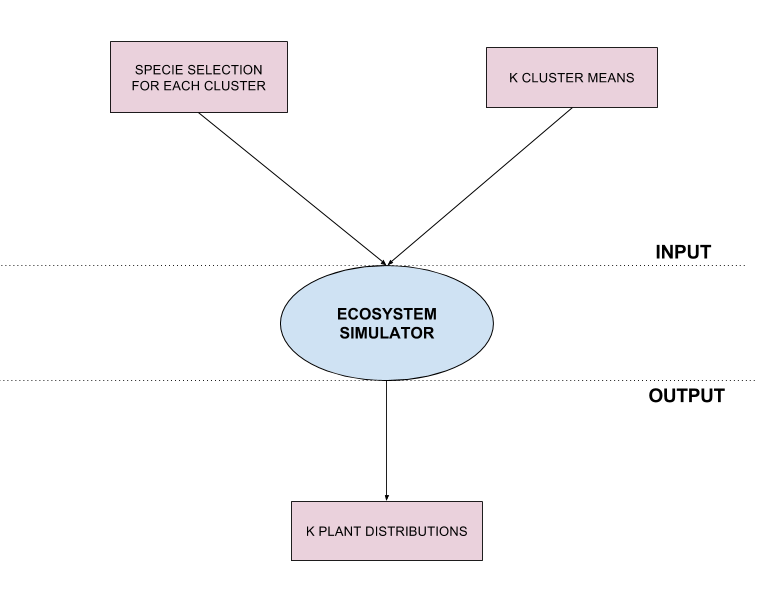
\includegraphics[scale=0.3]{system_overview_ecosystem_simulator.png}
	\caption{ Ecosystem simulator overview.}	
	\label{fig:system_overview_ecosystem_simulator}
\end{figure}

\section{Distribution Analyser and Reproducer}

Because the ecosystem simulator is computationally expensive, the simulation area is restricted to ten thousand square metres (hundred by hundred metres). In order to place vegetation in clusters with larger surface areas, radial distribution analysis and reproduction is performed. This technique analyses the variation in plant density over distance of an input exemplar in order to generate pair correlation histograms which are used to reproduce distributions matching the characteristics of the input exemplar. Because the reproduction is much less computationally costly than the ecosystem simulator, it is possible to efficiently produce distributions covering much larger areas. Figure \ref{fig:system_overview_distribution_analyser_and_reproducer} shows the input requirements and outputs of this component.

\begin{figure}
\center
	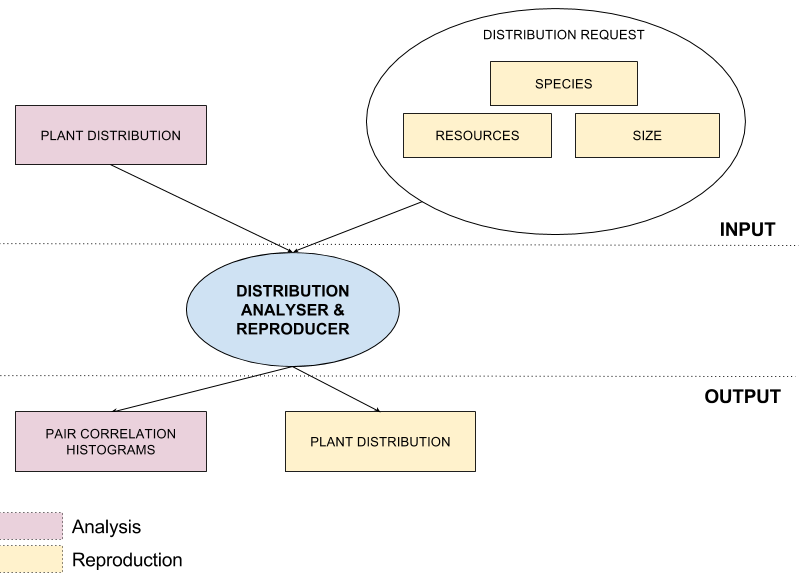
\includegraphics[scale=0.3]{system_overview_radial_distribution_analyzer_and_reproducer.png}
	\caption{ Distribution analyser and reproducer overview.}	
	\label{fig:system_overview_distribution_analyser_and_reproducer}
\end{figure}